% Options for packages loaded elsewhere
% Options for packages loaded elsewhere
\PassOptionsToPackage{unicode}{hyperref}
\PassOptionsToPackage{hyphens}{url}
%
\documentclass[
  indonesian,
  12pt,
  a4paper,
]{report}
\usepackage{xcolor}
\usepackage[top=4cm,bottom=3cm,left=4cm,right=3cm,headheight=15pt]{geometry}
\usepackage{amsmath,amssymb}
\setcounter{secnumdepth}{3}
\usepackage{iftex}
\ifPDFTeX
  \usepackage[T1]{fontenc}
  \usepackage[utf8]{inputenc}
  \usepackage{textcomp} % provide euro and other symbols
\else % if luatex or xetex
  \usepackage{unicode-math} % this also loads fontspec
  \defaultfontfeatures{Scale=MatchLowercase}
  \defaultfontfeatures[\rmfamily]{Ligatures=TeX,Scale=1}
\fi
\usepackage{lmodern}
\ifPDFTeX\else
  % xetex/luatex font selection
  \setmainfont[]{TeX Gyre Termes}
\fi
% Use upquote if available, for straight quotes in verbatim environments
\IfFileExists{upquote.sty}{\usepackage{upquote}}{}
\IfFileExists{microtype.sty}{% use microtype if available
  \usepackage[]{microtype}
  \UseMicrotypeSet[protrusion]{basicmath} % disable protrusion for tt fonts
}{}
\usepackage{setspace}
% Make \paragraph and \subparagraph free-standing
\makeatletter
\ifx\paragraph\undefined\else
  \let\oldparagraph\paragraph
  \renewcommand{\paragraph}{
    \@ifstar
      \xxxParagraphStar
      \xxxParagraphNoStar
  }
  \newcommand{\xxxParagraphStar}[1]{\oldparagraph*{#1}\mbox{}}
  \newcommand{\xxxParagraphNoStar}[1]{\oldparagraph{#1}\mbox{}}
\fi
\ifx\subparagraph\undefined\else
  \let\oldsubparagraph\subparagraph
  \renewcommand{\subparagraph}{
    \@ifstar
      \xxxSubParagraphStar
      \xxxSubParagraphNoStar
  }
  \newcommand{\xxxSubParagraphStar}[1]{\oldsubparagraph*{#1}\mbox{}}
  \newcommand{\xxxSubParagraphNoStar}[1]{\oldsubparagraph{#1}\mbox{}}
\fi
\makeatother


\usepackage{longtable,booktabs,array}
\newcounter{none} % for unnumbered tables
\usepackage{calc} % for calculating minipage widths
% Correct order of tables after \paragraph or \subparagraph
\usepackage{etoolbox}
\makeatletter
\patchcmd\longtable{\par}{\if@noskipsec\mbox{}\fi\par}{}{}
\makeatother
% Allow footnotes in longtable head/foot
\IfFileExists{footnotehyper.sty}{\usepackage{footnotehyper}}{\usepackage{footnote}}
\makesavenoteenv{longtable}
\usepackage{graphicx}
\makeatletter
\newsavebox\pandoc@box
\newcommand*\pandocbounded[1]{% scales image to fit in text height/width
  \sbox\pandoc@box{#1}%
  \Gscale@div\@tempa{\textheight}{\dimexpr\ht\pandoc@box+\dp\pandoc@box\relax}%
  \Gscale@div\@tempb{\linewidth}{\wd\pandoc@box}%
  \ifdim\@tempb\p@<\@tempa\p@\let\@tempa\@tempb\fi% select the smaller of both
  \ifdim\@tempa\p@<\p@\scalebox{\@tempa}{\usebox\pandoc@box}%
  \else\usebox{\pandoc@box}%
  \fi%
}
% Set default figure placement to htbp
\def\fps@figure{htbp}
\makeatother


% definitions for citeproc citations
\NewDocumentCommand\citeproctext{}{}
\NewDocumentCommand\citeproc{mm}{%
  \begingroup\def\citeproctext{#2}\cite{#1}\endgroup}
\makeatletter
 % allow citations to break across lines
 \let\@cite@ofmt\@firstofone
 % avoid brackets around text for \cite:
 \def\@biblabel#1{}
 \def\@cite#1#2{{#1\if@tempswa , #2\fi}}
\makeatother
\newlength{\cslhangindent}
\setlength{\cslhangindent}{1.5em}
\newlength{\csllabelwidth}
\setlength{\csllabelwidth}{3em}
\newenvironment{CSLReferences}[2] % #1 hanging-indent, #2 entry-spacing
 {\begin{list}{}{%
  \setlength{\itemindent}{0pt}
  \setlength{\leftmargin}{0pt}
  \setlength{\parsep}{0pt}
  % turn on hanging indent if param 1 is 1
  \ifodd #1
   \setlength{\leftmargin}{\cslhangindent}
   \setlength{\itemindent}{-1\cslhangindent}
  \fi
  % set entry spacing
  \setlength{\itemsep}{#2\baselineskip}}}
 {\end{list}}
\usepackage{calc}
\newcommand{\CSLBlock}[1]{\hfill\break\parbox[t]{\linewidth}{\strut\ignorespaces#1\strut}}
\newcommand{\CSLLeftMargin}[1]{\parbox[t]{\csllabelwidth}{\strut#1\strut}}
\newcommand{\CSLRightInline}[1]{\parbox[t]{\linewidth - \csllabelwidth}{\strut#1\strut}}
\newcommand{\CSLIndent}[1]{\hspace{\cslhangindent}#1}

\ifLuaTeX
\usepackage[bidi=basic,shorthands=off,provide=*]{babel}
\else
\usepackage[bidi=default,shorthands=off,provide=*]{babel}
\fi
\ifPDFTeX
\else
\babelfont{rm}[]{TeX Gyre Termes}
\fi
\ifLuaTeX
  \usepackage{selnolig} % disable illegal ligatures
\fi


\setlength{\emergencystretch}{3em} % prevent overfull lines

\providecommand{\tightlist}{%
  \setlength{\itemsep}{0pt}\setlength{\parskip}{0pt}}



 


% ============================================================
% meta.tex  --  data diri & judul skripsi
% ============================================================
\usepackage{graphicx}

\newcommand{\judul}{MODEL TEREDUKSI DUA FASA PIPA KALOR NATRIUM UNTUK PENDINGINAN PASIF REAKTOR ANTARIKSA INDONESIA: VALIDASI TERHADAP UJI KRUSTY DAN APLIKASI PADA TERAS 61 PIN 500~kWth}
\newcommand{\judulinggris}{REDUCED-ORDER TWO-PHASE MODEL OF A SODIUM HEAT PIPE FOR PASSIVE COOLING OF THE INDONESIAN SPACE REACTOR: VALIDATION AGAINST THE KRUSTY TEST AND APPLICATION TO A 61-PIN 500~kWth CORE}

\newcommand{\nama}{Muhammad Naufal Tamimi}
\newcommand{\nim}{20/456315/TK/50445}
\newcommand{\tahundaftar}{2020}
\newcommand{\tahun}{2026}

\newcommand{\prodi}{Teknik Nuklir}
\newcommand{\prodien}{Nuclear Engineering}

\newcommand{\kotatanggal}{Yogyakarta, \today}
\newcommand{\tglujian}{tanggal bulan tahun ujian}
\newcommand{\tglpengesahan}{DD BULAN TAHUN}
\newcommand{\tglujianinggris}{Month Date, year}

\newcommand{\pembimbingutama}{Nama Lengkap Pembimbing Utama}
\newcommand{\pembimbingpendamping}{Nama Lengkap Pembimbing Pendamping}
\newcommand{\ketuasidang}{Nama Lengkap Ketua Sidang}
\newcommand{\pengujiutama}{Nama Lengkap Penguji Utama}
\newcommand{\anggotapenguji}{Nama Lengkap Anggota Penguji}

\newcommand{\ketuadepartemen}{Dr. Ir. Alexander Agung, S.T., M.Sc., IPU}
\newcommand{\nipketua}{19720916 199803 1002}

\newcommand{\logougm}{%
  \IfFileExists{fig/Lambang-UGM-hitam.png}%
    {
\includegraphics[width=5.5cm]{fig/Lambang-UGM-hitam.png}}%
    {\fbox{\parbox[c][5.5cm][c]{5.5cm}{\centering\small Letakkan logo UGM}}}
}
% ============================================================
% header.tex -- aturan tipografi mengikuti Template Skripsi 2023/2025 DTNTF UGM
% ============================================================
\usepackage{titlesec}
\usepackage{titletoc}
\usepackage{fancyhdr}
\usepackage{caption}
\usepackage{etoolbox}
\usepackage{setspace}
\usepackage{enumitem}
\usepackage{xcolor}
\usepackage{array}
\usepackage{indentfirst}
\usepackage{fvextra}
\AtBeginEnvironment{longtable}{\small}
\setlength{\LTcapwidth}{\textwidth}
\DefineVerbatimEnvironment{Highlighting}{Verbatim}{breaklines,commandchars=\\\{\}}
\fvset{fontsize=\footnotesize}

% Alinea rata kiri-kanan, awal alinea menjorok 1,27 cm (sama dengan templat)
\setlength{\parindent}{1.27cm}
\setlength{\parskip}{0pt}

% ---------- Penomoran ----------
% Bab: "BAB I"; subbab: I.1, I.2.1 (Romawi.Arab)
% Gambar/Tabel/Persamaan: Arab per bab (5.1); di lampiran: A.1
\renewcommand{\thechapter}{BAB~\Roman{chapter}}
\renewcommand{\thesection}{\Roman{chapter}.\arabic{section}}
\renewcommand{\thesubsection}{\thesection.\arabic{subsection}}
\renewcommand{\thesubsubsection}{\thesubsection.\arabic{subsubsection}}
\renewcommand{\thefigure}{\arabic{chapter}.\arabic{figure}}
\renewcommand{\thetable}{\arabic{chapter}.\arabic{table}}
\renewcommand{\theequation}{\arabic{chapter}.\arabic{equation}}

% ---------- Judul bab / subbab ----------
% Judul bab: "BAB I" lalu judul, HURUF KAPITAL, tebal, rata tengah
\titleformat{\chapter}[display]
  {\normalfont\bfseries\centering\setstretch{1}}{\thechapter}{4pt}{\MakeUppercase}
\titleformat{name=\chapter,numberless}[block]
  {\normalfont\bfseries\centering\setstretch{1}}{}{0pt}{\MakeUppercase}
\titlespacing*{\chapter}{0pt}{0pt}{22pt}

% Subbab: "I.1. Judul", tebal, rata kiri, Title Case (diketik manual)
\titleformat{\section}{\normalfont\bfseries\setstretch{1}}{\thesection.}{0.6em}{}
\titleformat{\subsection}{\normalfont\bfseries\setstretch{1}}{\thesubsection.}{0.6em}{}
\titleformat{\subsubsection}{\normalfont\bfseries\setstretch{1}}{\thesubsubsection.}{0.6em}{}
\titlespacing*{\section}{0pt}{16pt}{8pt}
\titlespacing*{\subsection}{0pt}{14pt}{8pt}
\titlespacing*{\subsubsection}{0pt}{12pt}{8pt}

% ---------- Daftar isi ----------
\titlecontents{chapter}[0pt]{\addvspace{4pt}}
  {\thecontentslabel\ \ }{}{\titlerule*[.5pc]{.}\contentspage}
\titlecontents{section}[1cm]{}
  {\thecontentslabel.\ \ }{}{\titlerule*[.5pc]{.}\contentspage}
\titlecontents{subsection}[2cm]{}
  {\thecontentslabel.\ \ }{}{\titlerule*[.5pc]{.}\contentspage}
% Tingkat khusus untuk LAMPIRAN A, B, ... (menjorok di bawah entri "LAMPIRAN")
\titlecontents{appchapter}[1cm]{}
  {\thecontentslabel\ \ }{}{\titlerule*[.5pc]{.}\contentspage}

\newcommand{\newaddcontentsline}[3]{%
  \ifstrequal{#1}{toc}%
    {\ifstrequal{#2}{chapter}%
      {\origaddcontentsline{toc}{appchapter}{#3}}%
      {\origaddcontentsline{#1}{#2}{#3}}}%
    {\origaddcontentsline{#1}{#2}{#3}}}
\newcommand{\appendixtoc}{%
  \let\origaddcontentsline\addcontentsline
  \let\addcontentsline\newaddcontentsline}

% ---------- Nomor halaman ----------
% Tengah bawah di semua halaman (sesuai templat)
\pagestyle{fancy}
\fancyhf{}
\fancyfoot[C]{\thepage}
\renewcommand{\headrulewidth}{0pt}
\fancypagestyle{plain}{\fancyhf{}\fancyfoot[C]{\thepage}\renewcommand{\headrulewidth}{0pt}}

% ---------- Judul gambar/tabel ----------
% Gambar: judul di bawah, "Gambar 5.1." label tebal, baris lanjutan menggantung.
% Tabel: judul di atas; satu baris -> rata tengah, lebih dari satu baris -> rata kiri-kanan.
\captionsetup{font={stretch=1}, labelfont=bf, labelsep=period,
              singlelinecheck=off, justification=justified, format=hang}
\captionsetup[table]{singlelinecheck=on}
\DeclareCaptionListFormat{gambarlist}{\figurename~#1#2.}
\DeclareCaptionListFormat{tabellist}{\tablename~#1#2.}
\captionsetup[figure]{listformat=gambarlist}
\captionsetup[table]{listformat=tabellist}
\makeatletter
\renewcommand*{\l@figure}{\@dottedtocline{1}{0em}{6em}}
\renewcommand*{\l@table}{\@dottedtocline{1}{0em}{6em}}
\makeatother

% ---------- Daftar (rincian): nomor menjorok 0,6 cm, teks 1,27 cm ----------
\setlist{leftmargin=1.27cm, labelsep=0.2cm, align=right, topsep=2pt}

% ---------- Daftar pustaka: spasi 1 ----------
\AtBeginEnvironment{CSLReferences}{\singlespacing}
\makeatletter
\@ifpackageloaded{caption}{}{\usepackage{caption}}
\AtBeginDocument{%
\ifdefined\contentsname
  \renewcommand*\contentsname{Daftar Isi}
\else
  \newcommand\contentsname{Daftar Isi}
\fi
\ifdefined\listfigurename
  \renewcommand*\listfigurename{Daftar Gambar}
\else
  \newcommand\listfigurename{Daftar Gambar}
\fi
\ifdefined\listtablename
  \renewcommand*\listtablename{Daftar Tabel}
\else
  \newcommand\listtablename{Daftar Tabel}
\fi
\ifdefined\figurename
  \renewcommand*\figurename{Gambar}
\else
  \newcommand\figurename{Gambar}
\fi
\ifdefined\tablename
  \renewcommand*\tablename{Tabel}
\else
  \newcommand\tablename{Tabel}
\fi
}
\@ifpackageloaded{float}{}{\usepackage{float}}
\floatstyle{ruled}
\@ifundefined{c@chapter}{\newfloat{codelisting}{h}{lop}}{\newfloat{codelisting}{h}{lop}[chapter]}
\floatname{codelisting}{Daftar}
\newcommand*\listoflistings{\listof{codelisting}{Daftar Daftar}}
\makeatother
\makeatletter
\makeatother
\makeatletter
\@ifpackageloaded{caption}{}{\usepackage{caption}}
\@ifpackageloaded{subcaption}{}{\usepackage{subcaption}}
\makeatother
\usepackage{bookmark}
\IfFileExists{xurl.sty}{\usepackage{xurl}}{} % add URL line breaks if available
\urlstyle{same}
% fallback for those not using the hyperref driver hyperxmp:
\makeatletter
\@ifundefined{xmpquote}{\newcommand{\xmpquote}[1]{#1}}{}
\makeatother
\hypersetup{
  pdflang={id},
  hidelinks,
  pdfcreator={LaTeX via pandoc}}


\author{}
\date{}
\begin{document}


\setstretch{1.43}
\chapter{DASAR TEORI}\label{dasar-teori}

\section{Skema dan Asumsi Model}\label{skema-dan-asumsi-model}

Pipa kalor yang dimodelkan berbentuk silinder dengan tiga zona aksial:
evaporator sepanjang \(L_e\) tempat kalor masuk, zona adiabatik
sepanjang \(L_a\), dan kondensor sepanjang \(L_c\) tempat kalor keluar.
Secara radial, pipa tersusun dari selubung logam, sumbu berpori jenuh
natrium cair, dan inti uap di bagian tengah (Gambar 3.1).

\begin{figure}[htbp]

\centering{

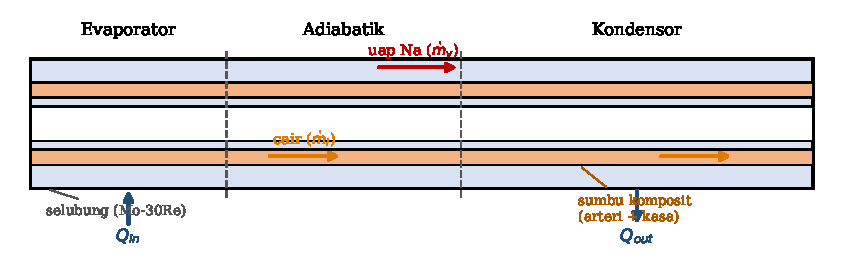
\includegraphics[width=0.9\linewidth,height=\textheight,keepaspectratio]{figures/skema_pipa_kalor.pdf}

}

\caption{\label{fig-skema}Skema pipa kalor natrium in-pin beserta arah
aliran uap dan cairan.}

\end{figure}%

Model dibangun atas lima asumsi yang perlu dinyatakan sejak awal karena
membatasi keberlakuannya.

\begin{enumerate}
\def\labelenumi{\arabic{enumi}.}
\tightlist
\item
  Aliran tunak (\emph{steady state}). Tidak ada suku akumulasi massa,
  momentum, maupun energi.
\item
  Uap berada dalam kesetimbangan saturasi lokal, sehingga
  \(T(z) = T_{sat}(P_v(z))\). Asumsi ini wajar untuk pipa kalor logam
  cair karena laju penguapan dan pengembunan jauh lebih cepat daripada
  transpor aksial.
\item
  Aliran uap satu dimensi aksial, seragam pada setiap penampang, dengan
  faktor gesek Darcy yang bergantung pada bilangan Reynolds lokal.
\item
  Sumbu berpori jenuh sempurna; aliran cairan mengikuti hukum Darcy yang
  diperluas dengan suku inersia Ergun.
\item
  Hambatan termal radial dihitung dengan jaringan satu dimensi,
  sedangkan konduksi aksial pada selubung diabaikan karena rasio panjang
  terhadap tebal dinding sangat besar.
\end{enumerate}

\section{Sifat Termofisika Natrium}\label{sifat-termofisika-natrium}

Sifat natrium cair dan uap dievaluasi dari korelasi Fink dan Leibowitz
{[}1{]} beserta korelasi pelengkap dari Faghri {[}2{]}. Densitas cairan
mengikuti hubungan linear

\begin{equation}\protect\phantomsection\label{eq-rhol}{\rho_l(T) = 1014 - 0{,}235\,T \quad [\mathrm{kg/m^3}]}\end{equation}

yang berlaku dalam 1\% pada rentang 400--1400 K. Viskositas dinamis
cairan dinyatakan sebagai

\begin{equation}\protect\phantomsection\label{eq-mul}{\ln \mu_l = -6{,}4406 - 0{,}3958 \ln T + \frac{556{,}835}{T} \quad [\mathrm{Pa\cdot s}]}\end{equation}

Tegangan permukaan mengikuti bentuk Watson yang dipatri pada temperatur
kritis \(T_c = 2503{,}7\) K,

\begin{equation}\protect\phantomsection\label{eq-sigma}{\sigma(T) = 0{,}2405 \left(1 - \frac{T}{T_c}\right)^{1{,}126} \quad [\mathrm{N/m}]}\end{equation}

dan kalor laten penguapan mengikuti bentuk serupa,

\begin{equation}\protect\phantomsection\label{eq-hfg}{h_{fg}(T) = 4{,}76 \times 10^{6} \left(1 - \frac{T}{T_c}\right)^{0{,}38} \quad [\mathrm{J/kg}]}\end{equation}

Persoalan muncul pada tekanan uap jenuh. Korelasi yang lazim dikutip
untuk natrium ditulis dalam bentuk tertutup dengan konstanta yang
berbeda-beda antar sumber, sehingga pada 1000 K hasilnya dapat berbeda
lebih dari satu orde besaran. Karena tekanan uap menentukan densitas uap
dan melalui densitas itu menentukan batas sonik, kesalahan pada besaran
ini akan merambat ke seluruh kesimpulan desain.

Untuk menghindari inkonsistensi tersebut, penelitian ini tidak memakai
korelasi tertutup, melainkan mengintegrasikan persamaan
Clausius--Clapeyron dengan kalor laten pada (Persamaan~\ref{eq-hfg}),

\begin{equation}\protect\phantomsection\label{eq-clapeyron}{\frac{d \ln P_{sat}}{dT} = \frac{h_{fg}(T)}{R_g T^{2}}}\end{equation}

dari titik didih normal \(T_b = 1156{,}2\) K tempat
\(P_{sat} = 101{,}325\) kPa, dengan \(R_g = R_u/M_{Na} = 361{,}66\)
J/(kg·K). Integrasi numerik dilakukan pada grid 0,25 K menggunakan
aturan trapesium. Cara ini menjamin bahwa kurva tekanan uap dan kurva
kalor laten yang dipakai model saling konsisten secara termodinamika.
Hasilnya adalah \(P_{sat}(1000\ \mathrm{K}) = 24{,}07\) kPa dan
\(P_{sat}(1075\ \mathrm{K}) = 50{,}1\) kPa.

Densitas uap dihitung dengan hukum gas ideal untuk natrium monomer,
\(\rho_v = P_v/(R_g T)\). Koreksi dimerisasi diabaikan; pada 1000--1100
K fraksi dimer natrium masih di bawah 8\%, sehingga kesalahan densitas
yang ditimbulkan tetap lebih kecil daripada ketidakpastian korelasi
tekanan uap itu sendiri.

\begin{figure}[htbp]

\centering{

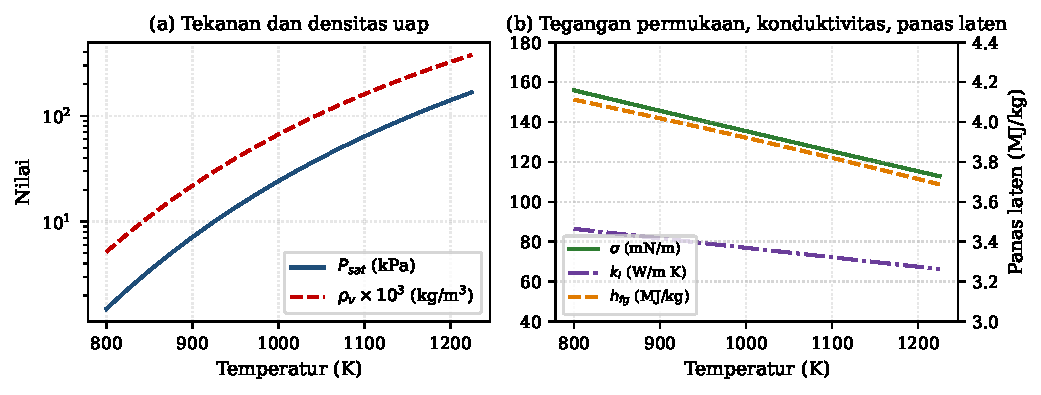
\includegraphics[width=0.95\linewidth,height=\textheight,keepaspectratio]{figures/sifat_natrium.pdf}

}

\caption{\label{fig-sifat}Sifat termofisika natrium jenuh pada rentang
operasi reaktor antariksa: (a) tekanan uap jenuh dan densitas uap; (b)
tegangan permukaan, konduktivitas termal, dan kalor laten.}

\end{figure}%

\begin{longtable}[]{@{}
  >{\centering\arraybackslash}p{(\linewidth - 14\tabcolsep) * \real{0.1250}}
  >{\centering\arraybackslash}p{(\linewidth - 14\tabcolsep) * \real{0.1250}}
  >{\centering\arraybackslash}p{(\linewidth - 14\tabcolsep) * \real{0.1250}}
  >{\centering\arraybackslash}p{(\linewidth - 14\tabcolsep) * \real{0.1250}}
  >{\centering\arraybackslash}p{(\linewidth - 14\tabcolsep) * \real{0.1250}}
  >{\centering\arraybackslash}p{(\linewidth - 14\tabcolsep) * \real{0.1250}}
  >{\centering\arraybackslash}p{(\linewidth - 14\tabcolsep) * \real{0.1250}}
  >{\centering\arraybackslash}p{(\linewidth - 14\tabcolsep) * \real{0.1250}}@{}}
\caption{Sifat termofisika natrium jenuh pada rentang operasi reaktor
antariksa.}\label{tbl-sifat}\tabularnewline
\toprule\noalign{}
\begin{minipage}[b]{\linewidth}\centering
\(T\) (K)
\end{minipage} & \begin{minipage}[b]{\linewidth}\centering
\(P_{sat}\) (kPa)
\end{minipage} & \begin{minipage}[b]{\linewidth}\centering
\(\rho_l\) (kg/m³)
\end{minipage} & \begin{minipage}[b]{\linewidth}\centering
\(\rho_v\) (kg/m³)
\end{minipage} & \begin{minipage}[b]{\linewidth}\centering
\(\mu_l\) (µPa·s)
\end{minipage} & \begin{minipage}[b]{\linewidth}\centering
\(h_{fg}\) (MJ/kg)
\end{minipage} & \begin{minipage}[b]{\linewidth}\centering
\(\sigma\) (mN/m)
\end{minipage} & \begin{minipage}[b]{\linewidth}\centering
\(k_l\) (W/m·K)
\end{minipage} \\
\midrule\noalign{}
\endfirsthead
\toprule\noalign{}
\begin{minipage}[b]{\linewidth}\centering
\(T\) (K)
\end{minipage} & \begin{minipage}[b]{\linewidth}\centering
\(P_{sat}\) (kPa)
\end{minipage} & \begin{minipage}[b]{\linewidth}\centering
\(\rho_l\) (kg/m³)
\end{minipage} & \begin{minipage}[b]{\linewidth}\centering
\(\rho_v\) (kg/m³)
\end{minipage} & \begin{minipage}[b]{\linewidth}\centering
\(\mu_l\) (µPa·s)
\end{minipage} & \begin{minipage}[b]{\linewidth}\centering
\(h_{fg}\) (MJ/kg)
\end{minipage} & \begin{minipage}[b]{\linewidth}\centering
\(\sigma\) (mN/m)
\end{minipage} & \begin{minipage}[b]{\linewidth}\centering
\(k_l\) (W/m·K)
\end{minipage} \\
\midrule\noalign{}
\endhead
\bottomrule\noalign{}
\endlastfoot
800 & 1,49 & 826 & 0,0051 & 227,1 & 4,11 & 155,9 & 86,5 \\
900 & 7,10 & 802 & 0,0218 & 200,6 & 4,02 & 145,6 & 81,8 \\
1.000 & 24,07 & 779 & 0,0666 & 180,8 & 3,92 & 135,5 & 77,0 \\
1.100 & 63,73 & 756 & 0,1602 & 165,6 & 3,82 & 125,4 & 72,2 \\
1.200 & 140,37 & 732 & 0,3234 & 153,3 & 3,71 & 115,3 & 67,5 \\
\end{longtable}

\section{Momentum Uap Kompresibel Satu
Dimensi}\label{momentum-uap-kompresibel-satu-dimensi}

Laju alir massa uap pada setiap posisi aksial ditentukan oleh fluks
penguapan dan pengembunan. Dengan \(Q\) sebagai daya yang ditranspor dan
\(h_{fg}\) dievaluasi pada temperatur kondensor,

\begin{equation}\protect\phantomsection\label{eq-mdot}{\dot m_v(z) = \frac{Q}{h_{fg}} \cdot m(z), \qquad
m(z) = \begin{cases} z/L_e, & 0 \le z \le L_e \\ 1, & L_e < z \le L_e + L_a \\ 1 - (z - L_e - L_a)/L_c, & z > L_e + L_a \end{cases}}\end{equation}

Momentum uap diselesaikan dari persamaan Navier--Stokes satu dimensi
yang dirata-ratakan pada penampang, dengan suku gesekan dinding dan suku
fluks momentum,

\begin{equation}\protect\phantomsection\label{eq-momentum}{\frac{dP_v}{dz} = -\frac{f_v \rho_v u_v^{2}}{2 D_v} - \beta \frac{d(\rho_v u_v^{2})}{dz}}\end{equation}

dengan \(u_v = \dot m_v/(\rho_v A_v)\) dan \(D_v = 2 r_v\). Faktor gesek
Darcy mengikuti rezim aliran,

\begin{equation}\protect\phantomsection\label{eq-fv}{f_v = \begin{cases} 64/Re_v, & Re_v < 2300 \\ 0{,}3164\,Re_v^{-0{,}25}, & Re_v \ge 2300 \end{cases}, \qquad Re_v = \frac{\rho_v u_v D_v}{\mu_v}}\end{equation}

Koefisien \(\beta\) membedakan injeksi massa pada evaporator
(\(\beta = 1\)) dari pengisapan massa pada kondensor
(\(\beta = 0{,}65\)). Perbedaan ini penting: pada evaporator, penambahan
massa radial mempercepat aliran aksial sehingga menambah rugi tekanan,
sedangkan pada kondensor pengisapan memperlambat aliran sehingga terjadi
pemulihan tekanan parsial {[}2{]}.

Karena \(T\) dan \(P\) terikat oleh kesetimbangan saturasi,
(Persamaan~\ref{eq-momentum}) merupakan persamaan diferensial biasa
untuk \(P_v(z)\) saja. Persamaan tersebut diintegrasikan mundur dari
\(z = L\), tempat \(P_v = P_{sat}(T_c)\) dan \(u_v = 0\), menuju
\(z = 0\) dengan metode Runge--Kutta orde empat pada 240 titik grid.
Hasilnya adalah profil tekanan, temperatur, kecepatan, dan bilangan Mach
sepanjang pipa.

Bilangan Mach lokal dihitung dengan kecepatan suara uap monatomik,

\begin{equation}\protect\phantomsection\label{eq-mach}{c_s = \sqrt{\gamma R_g T}, \qquad Ma(z) = \frac{u_v(z)}{c_s}, \qquad \gamma = 5/3}\end{equation}

\section{Aliran Balik Cairan pada Sumbu
Komposit}\label{aliran-balik-cairan-pada-sumbu-komposit}

Cairan yang terkondensasi di kondensor harus kembali ke evaporator
melalui sumbu berpori. Untuk sumbu komposit yang terdiri atas arteri
annular terbuka dan lapisan kasa halus pembentuk meniskus, aliran cairan
mengikuti

\begin{equation}\protect\phantomsection\label{eq-darcy}{\frac{dP_l}{dz} = \frac{\mu_l \dot m_l}{\rho_l A_w K} + \frac{\rho_l g \sin\psi}{1}}\end{equation}

dengan \(A_w\) luas penampang aliran efektif sumbu dan \(K\)
permeabilitas. Suku inersia Ergun diabaikan karena bilangan Reynolds
cairan dalam pori berorde jauh di bawah satu untuk seluruh kasus yang
ditinjau. Kekekalan massa memberikan \(\dot m_l(z) = \dot m_v(z)\),
sehingga profil laju alir cairan identik dengan profil uap.

Nilai permeabilitas ditentukan oleh struktur sumbu. Untuk arteri annular
terbuka dengan celah radial \(b\), pendekatan saluran sempit memberikan
\(K \approx b^{2}/8\); untuk \(b = 0{,}8\) mm diperoleh
\(K \approx 8 \times 10^{-8}\) m\(^{2}\), jauh lebih besar daripada
sumbu kasa tunggal yang hanya berkisar \(10^{-11}\)--\(10^{-10}\)
m\(^{2}\) {[}3{]}. Dalam model ini dipakai nilai konservatif
\(K = 5 \times 10^{-9}\) m\(^{2}\) untuk memperhitungkan penyempitan
akibat dinding arteri dan sisa kasa.

Tekanan kapiler yang tersedia pada meniskus mengikuti persamaan
Young--Laplace,

\begin{equation}\protect\phantomsection\label{eq-laplace}{\Delta P_{c}(z) = P_v(z) - P_l(z) \le \Delta P_{c,maks} = \frac{2\sigma}{r_{eff}}}\end{equation}

dengan \(r_{eff}\) jari-jari pori efektif kasa pembentuk meniskus dan
sudut kontak diambil nol karena natrium membasahi logam refraktori
secara sempurna. Syarat operasi tunak adalah

\begin{equation}\protect\phantomsection\label{eq-neraca-tekanan}{\Delta P_{c,maks} \ge \Delta P_v + \Delta P_l + \Delta P_g}\end{equation}

dengan \(\Delta P_v\) rugi tekanan uap total, \(\Delta P_l\) rugi
tekanan cairan total, dan \(\Delta P_g = \rho_l g L \sin\psi\) komponen
hidrostatik.

\section{Batas-Batas Operasi}\label{batas-batas-operasi}

\subsection{Batas Kapiler}\label{batas-kapiler}

Batas kapiler tercapai ketika kebutuhan tekanan sirkulasi menyamai
tekanan kapiler maksimum. Karena \(\Delta P_v\) tumbuh sebanding
\(Q^{2}\) sedangkan \(\Delta P_l\) sebanding \(Q\), batas ini ditentukan
dengan metode bagi dua (\emph{bisection}) pada \(Q\) hingga
(Persamaan~\ref{eq-neraca-tekanan}) terpenuhi sebagai persamaan.
Pendekatan ini lebih akurat daripada rumus tertutup
\(Q_{cap} = (\Delta P_{c,maks} - \Delta P_g)/[(F_l + F_v)L_{eff}]\) yang
mengabaikan ketergantungan \(F_v\) pada \(Q\).

\subsection{Batas Sonik}\label{batas-sonik}

Ketika temperatur rendah, densitas uap sangat kecil sehingga kecepatan
uap di ujung evaporator dapat mencapai kecepatan suara. Korelasi
Levy--Busse memberikan

\begin{equation}\protect\phantomsection\label{eq-sonic}{Q_{sonic} = A_v \rho_v h_{fg} \sqrt{\frac{\gamma R_g T}{2(\gamma + 1)}}}\end{equation}

Korelasi ini mengasumsikan densitas uap konstan sepanjang pipa. Model
ini juga menghitung bilangan Mach secara langsung dari
(Persamaan~\ref{eq-mach}), sehingga dapat diperiksa apakah korelasi
tersebut konservatif atau tidak.

\subsection{Batas Entrainment}\label{batas-entrainment}

Tetesan cairan terlepas dari permukaan meniskus ketika gaya geser uap
melampaui gaya tegangan permukaan. Kriteria Weber
\(We = \rho_v u_v^{2}(2 r_{eff})/\sigma \ge 1\) memberikan

\begin{equation}\protect\phantomsection\label{eq-ent}{Q_{ent} = A_v h_{fg} \sqrt{\frac{\sigma \rho_v}{2 r_{eff}}}}\end{equation}

\subsection{Batas Viskos}\label{batas-viskos}

Pada temperatur sangat rendah, gradien tekanan viskos dapat mencekik
aliran sebelum rezim sonik tercapai. Batas Busse untuk kasus ini adalah

\begin{equation}\protect\phantomsection\label{eq-visc}{Q_{visc} = \frac{r_v^{2} h_{fg} \rho_v P_{sat} A_v}{16 \mu_v L_{eff}}}\end{equation}

\subsection{Batas Pendidihan}\label{batas-pendidihan}

Jika fluks kalor radial terlalu tinggi, gelembung uap dapat terbentuk di
dalam pori dan mengisolasi dinding dari pasokan cairan. Ambang
terjadinya nukleasi pada rongga berjari-jari \(r_n\) adalah

\begin{equation}\protect\phantomsection\label{eq-boil}{\Delta T_{krit} = \frac{2 \sigma T_{sat}}{\rho_v h_{fg} r_n}, \qquad
Q_{boil} = \frac{2 \pi L_e k_{eff} \Delta T_{krit}}{\ln(r_i/r_v)}}\end{equation}

dengan \(k_{eff}\) konduktivitas efektif sumbu jenuh menurut model
Maxwell--Eucken dan \(r_n = 2{,}5\) µm.

Amplop operasi adalah nilai minimum dari kelima batas,

\begin{equation}\protect\phantomsection\label{eq-env}{Q_{env}(T) = \min\left(Q_{cap},\, Q_{sonic},\, Q_{ent},\, Q_{visc},\, Q_{boil}\right)}\end{equation}

\section{Jaringan Hambatan Termal
Radial}\label{jaringan-hambatan-termal-radial}

Beda temperatur antara dinding evaporator dan dinding kondensor terdiri
atas empat komponen: konduksi radial pada dinding evaporator, konduksi
radial pada sumbu, penurunan temperatur uap akibat gradien tekanan, dan
konduksi radial pada dinding kondensor. Masing-masing dinyatakan sebagai

\begin{equation}\protect\phantomsection\label{eq-rth}{R_{wall} = \frac{\ln(r_o/r_i)}{2\pi k_w L_e}, \quad
R_{wick} = \frac{\ln(r_i/r_v)}{2\pi k_{eff} L_e}, \quad
R_{vap} = \frac{8 \mu_v T}{\pi \rho_v^{2} h_{fg}^{2} r_v^{4}}}\end{equation}

Hambatan total pipa adalah
\(R_{th} = R_{wall} + R_{wick} + R_{cond,wall} + R_{vap}\), dan beda
temperatur totalnya \(\Delta T_{hp} = Q R_{th}\) ditambah penurunan
temperatur saturasi sepanjang inti uap.

\section{Konduksi Radial Pelet Uranium
Nitrida}\label{konduksi-radial-pelet-uranium-nitrida}

Pelet bahan bakar ISR berbentuk anular: panas dibangkitkan di dalam
annulus dan mengalir ke dalam menuju pipa kalor, sedangkan permukaan
luar pelet bersentuhan dengan kelongsong yang secara termal mendekati
adiabatik. Untuk pembangkitan volumetrik seragam \(q'''\) dan temperatur
permukaan dalam \(T_i\), solusi tunak persamaan konduksi satu dimensi
adalah

\begin{equation}\protect\phantomsection\label{eq-fuel}{T(r) = T_i + \frac{q'''}{2k}\left[r_o^{2}\ln\frac{r}{r_i} - \frac{r^{2} - r_i^{2}}{2}\right]}\end{equation}

sehingga kenaikan temperatur puncak di permukaan luar pelet, tempat
\(T\) maksimum, adalah

\begin{equation}\protect\phantomsection\label{eq-dtfuel}{\Delta T_{UN} = \frac{q'''}{2k_{UN}}\left[r_o^{2}\ln\frac{r_o}{r_i} - \frac{r_o^{2} - r_i^{2}}{2}\right]}\end{equation}

dengan \(q''' = Q_{pin}/[\pi(r_o^{2} - r_i^{2})H]\). Persamaan ini
mengabaikan ketergantungan \(k_{UN}\) pada temperatur dan gradasi
pembangkitan akibat \emph{burnup}; keduanya bersifat konservatif karena
menaikkan perkiraan temperatur puncak.

\section{Pengaruh Gravitasi dan Rezim
Mikrogravitasi}\label{pengaruh-gravitasi-dan-rezim-mikrogravitasi}

Komponen hidrostatik \(\Delta P_g = \rho_l g L \sin\psi\) hilang pada
\(g = 0\). Pada pengujian darat dengan evaporator di atas
(\(\psi = 90^\circ\)), suku ini mencapai sekitar 3,4 kPa untuk pipa
sepanjang 0,46 m pada 1075 K, yaitu sekitar 20\% dari tekanan kapiler
maksimum. Karena itu pengujian darat selalu memberikan batas operasi
yang lebih rendah daripada operasi sesungguhnya di orbit, dan perbedaan
tersebut harus diperhitungkan ketika hasil uji bumi dipakai untuk
merancang pipa kalor antariksa.

\section{Hipotesis}\label{hipotesis}

Berdasarkan tinjauan teoretis di atas, diajukan tiga hipotesis.

\begin{enumerate}
\def\labelenumi{\arabic{enumi}.}
\tightlist
\item
  Model tereduksi satu dimensi yang menggabungkan momentum uap
  kompresibel, filtrasi Darcy, dan jaringan hambatan termal mampu
  mereproduksi karakteristik beda temperatur pipa kalor KRUSTY dengan
  kesalahan rata-rata di bawah 10\% pada pengujian \emph{leave-one-out}.
\item
  Pada rentang temperatur kerja 1000--1150 K, mekanisme pembatas pipa
  kalor berukuran diameter luar 16--20 mm adalah batas entrainment,
  bukan batas kapiler sebagaimana lazim diasumsikan pada literatur pipa
  kalor logam cair.
\item
  Penggantian loop pompa Na-78K oleh pipa kalor natrium pada teras ISR
  500 kWth menghasilkan margin keselamatan positif untuk seluruh 61 pin,
  tetapi menuntut pengurangan volume bahan bakar lebih dari 20\% akibat
  pelebaran rongga tengah pin.
\end{enumerate}

\protect\phantomsection\label{refs}
\begin{CSLReferences}{0}{1}
\bibitem[\citeproctext]{ref-fink1995thermodynamic}
\CSLLeftMargin{{[}1{]} }%
\CSLRightInline{J. K. Fink dan L. Leibowitz. \emph{Thermodynamic and
Transport Properties of Sodium Liquid and Vapor}. Argonne, IL, Argonne
National Laboratory, 1995.}

\bibitem[\citeproctext]{ref-faghri1995heat}
\CSLLeftMargin{{[}2{]} }%
\CSLRightInline{A. Faghri. \emph{Heat Pipe Science and Technology}.
Washington, DC, Taylor \& Francis, 1995.}

\bibitem[\citeproctext]{ref-chi1976heat}
\CSLLeftMargin{{[}3{]} }%
\CSLRightInline{S. W. Chi. \emph{Heat Pipe Theory and Practice: A
Sourcebook}. Washington, DC, Hemisphere Publishing Corporation, 1976.}

\end{CSLReferences}




\end{document}
